\documentclass[a4paper]{article}
\usepackage[utf8]{inputenc}
\usepackage[russian,english]{babel}
\usepackage[T2A]{fontenc}
\usepackage[left=10mm, top=20mm, right=18mm, bottom=15mm, footskip=10mm]{geometry}
\usepackage{indentfirst}
\usepackage{amsmath,amssymb}
\usepackage[italicdiff]{physics}
\usepackage{graphicx}
\usepackage{caption}
\usepackage{float}
\usepackage[parfill]{parskip}
\usepackage[utf8]{inputenc}\newcommand{\approxtext}[1]{\ensuremath{\stackrel{\text{#1}}{\approx}}}
\graphicspath{{images/}}
\DeclareGraphicsExtensions{.pdf,.png,.jpg}
\usepackage{wrapfig}
\captionsetup{labelformat=empty}

\usepackage{caption}
\captionsetup[figure]{name=Рисунок}
\captionsetup[table]{name=Таблица}
  
\title{\textbf{Отчет о выполненой лабораторной работе 2.1.1}}
\date{}
\author{Котляров Михаил, Б01-402}



\begin{document}

\maketitle
	
	\section{Введение}
	
	\textbf{Цель работы:} измерить повышение температуры воздуха в зависимости от мощности
подводимого тепла и расхода при стационарном течении через трубу; исключив тепловые потери, по результатам измерений определить теплоёмкость воздуха при постоянном давлении.\\
	\textbf{Оборудование:} теплоизолированная стеклянная трубка; электронагреватель; источник питания постоянного тока; амперметр, вольтметр (цифровые мультиметры); термопара, подключенная к микровольтметру; компрессор; газовый счётчик;
секундомер.
	
	\section{Теоретические сведения}
Теплоёмкость тела в некотором процессе определяется как их отношение:
\begin{equation} \tag{1}
C = \frac{\delta Q}{dT}
\end{equation}

Рассмотрим газ, протекающий стационарно слева направо через трубу постоянного сечения, в которой установлен нагревательный элемент (см. рис. 1). Пусть за некоторое время $dt$ через калориметр прошла малая порция газа массой $dm=q \, dt$, где $q$ [кг/с] — массовый расход газа в трубе. Если мощность нагрева равна $N$, мощность тепловых потерь на обмен с окружающей средой $N_{\text{пот}}$, то порция
	получила тепло $\delta Q = (N-N_{\text{пот}})dt$. С другой стороны, по определению теплоёмкости (1): $\delta Q = c \, dm \Delta T$, где $\Delta T = T_{2}-T_{1}$ — приращение температуры	газа, и $c$ — удельная (на единицу массы) теплоёмкость газа в рассматриваемом процессе. При малых расходах газа и достаточно большом диаметре
	трубы перепад давления на её концах мал, поэтому можно принять, что $p_{1} \approx p_{2} = p_{0}$, где $p_{0}$ — атмосферное давление. Следовательно, в условиях опыта измеряется удельная теплоёмкость при постоянном давлении $c_{p}$. Таким образом, получаем 
\begin{equation*}
	c_{p} = \frac{N-N_{\text{пот}}}{q\Delta T}
	\eqno(2)
\end{equation*}

\begin{figure}[h!]
		\centering{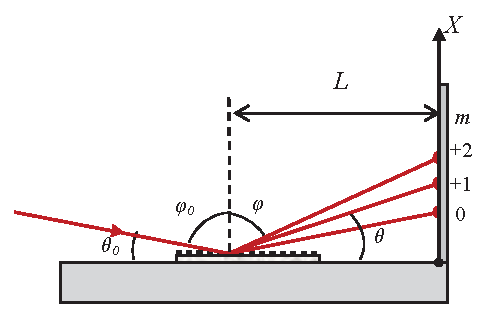
\includegraphics[width=0.5\textwidth]{Pictures/pic1.jpg}}
		\caption[]{\label{fig:1} Нагрев газа при течении по трубе}
	\end{figure}

\section{Экспериментальная установка}
Напряжение на нагревателе $U$ и ток $I$ через него регистрируются цифровыми
мультиметрами. Таким образом, мощность нагрева равна
\begin{equation*}
		N = UI
		\eqno(3)
\end{equation*}
\begin{figure}[h!]
	\centering{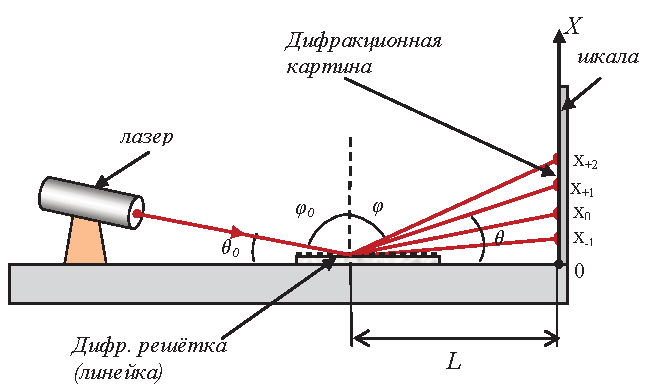
\includegraphics[width=0.5\textwidth]{Pictures/pic2.jpg}}
	\caption[]{\label{fig:2} Схема экспериментальной установки}
\end{figure}
Для измерения разности температур $\Delta T$ служит медно-константановая
термопара. Один спай термопары расположен в струе воздуха, входящего в
калориметр, и находится при комнатной температуре, а второй — в струе выходящего нагретого воздуха. Константановая проволока термопары расположена внутри калориметра, а медные проводники подключены к цифровому вольтметру. Возникающая в термопаре ЭДС $\varepsilon$ пропорциональна разности температур $\Delta T$ спаев: 
	\begin{equation*}
		\varepsilon =\beta \Delta T
		\eqno(4)
	\end{equation*}

где $\beta = 40.7 \frac{мкВ}{К}$ — чувствительность медно-константановой термопары в рабочем диапазоне температур (20–30 $^\circ C$ ). ЭДС регистрируется с помощью микровольтметра.

Объёмный расход равен $\frac{\Delta V}{\Delta t} $, массовый расход может быть найден как 
\begin{equation*}
	q = \rho_{0} \frac{\Delta V}{\Delta t}
	\eqno(5)
\end{equation*}

где $\rho_{0}$ — плотность воздуха при комнатной температуре, которая в свою очередь может быть получена из уравнения Менделеева–Клапейрона: $\rho_{0}= \frac{\mu p_{0} }{R T_{0}},$ где $p_{0}$ — атмосферное давление, $T_{0}$ — комнатная температура (в Кельвинах), $\mu = 29,0 {г/моль}$ — средняя молярная масса (сухого) воздуха.
Можно предположить, что при небольшом нагреве ($\Delta T \ll T_{0}$) мощность потерь тепла $N_{пот}$ прямо пропорциональна разности температур:
\begin{equation*}
	N_{\text{пот}} = \alpha \Delta T
	\eqno(6)
\end{equation*}

где $\alpha$ — некоторая константа. При этом условии основное соотношение (2) принимает вид 
\begin{equation*}
	N = (c_{p}q +\alpha)\Delta T
	\eqno(7)
\end{equation*}

Следовательно, при фиксированном расходе воздуха ($q = const$) подводимая мощность и разность температур связаны прямой пропорциональностью ($\Delta T(N)$ -- линейная функция).

\section{Приборы и данные}
\begin{itemize}
    \item вольтметр, измеряющий напряжение на термопаре, погрешность -- 0,0035\%
    \item вольтметр, погрешность 0,5\%
    \item Два мультиметра, погрешность измерения постоянного напряжения 0,03\%, погрешность мзмерения постоянного тока 0,2\%
    \item Термогигрометр с функцией отображения давления, погрешность измерения температуры $\sigma_{T} = \pm 0,4 ^\circ C$, давления -- $\sigma_{p} = \pm 300 \text{Па}$
    \item Газосчетчик, класс точности -- 1,0
\end{itemize}

\section{Выполнение}

\begin{enumerate}
\item Подготовим к работе газовый счетчик: проверим, заполнен ли он водой, установим счетчик по уровню. Убедимся, что при постоянном расходе его стрелка вращается равномерно.
\item Включим вольтметр и проверим, что напряжение на термопаре равно нулю.
\item Температура в комнате $T = 296,4\pm0,4K$, давление $p = 101050\pm300 \text{Па}$, влажность 29,5\%
\item Определим плотность воздуха в помещении
\begin{equation*}
	\rho = \frac{p\mu}{RT} \stackrel{}{\approx} 1,1897 \pm 0,0038\frac{\text{г}}{\text{л}}
\end{equation*}
Массовый расход $q$
\begin{equation*}
	q_1 = \rho \frac{\Delta V}{\Delta t} = \frac{\mu p}{RT} \frac{\Delta V}{\Delta t_1} \stackrel{}{\approx} 0,1879 \pm 0,0003 \frac{\text{г}}{\text{c}}
\end{equation*}
Считая воздух идеальным двухатомным газом, определим теоретическое значение удельной теплоемкости при постоянном давлении
\begin{equation*}
	c_{p}^{теор} = \frac{3.5R}{\mu} \approx 1,003 \frac{\text{Дж}}{\text{г}\cdot K}
\end{equation*}
Оценим величину тока нагревателя, требуемого для нагрева воздуха на $\Delta T = 1 ^\circ C$
\begin{equation*}
	N \approx  c_{p}^{теор} q  \Delta T \approx 0,189 \text{Вт}
\end{equation*}
Сопротивление проволоки нагревателя $R = 37 \text{ Ом}$, искомый ток $I = \sqrt{\frac{N}{R}} \approx 71,47 \text{ мА}$
\item Проведем измерение зависимости разности температур от мощности нагревателя $\Delta T(N)$ при расходе $q_1 = 0,1879 \pm 0,0006 \text{ }\frac{\text{г}}{\text{c}} (\varepsilon = 0,33\%)$.
\begin{table}[h!] 
			\caption{Измерение $\Delta T (N) \; {при} \; q_1 = 0,1879 \pm 0,0006 \frac{\text{г}}{\text{c}}$}
			\begin{center}
				\begin{tabular}{|*{6}{c|}}
					\hline
					\textnumero & $U, \text{B} $ & $\varepsilon,  \text{мВ}$ & $I, \text{мА}$ & $\Delta T, ^\circ\text{C}$ & $N,  \text{Вт} $\\ \hline
					1	& 2,55	 & 0,039 & 71,47	 & 0,96 & 0,182\\ \hline
					2	& 3,62 & 	0,076	& 101,14	&1,87&	0,366\\ \hline
					3	&5,05&	0,143	&141,31	&3,51	&0,714\\ \hline
					4	&	6,27&	0,217	&175,36&	5,33&	1,100\\ \hline
					5	&6,95&	0,283	&199,9	&6,95&	1,389\\ \hline
					6	&7,78&	0,35&	223,3	&8,60&	1,737\\ \hline
				\end{tabular}
			\end{center}
		\end{table}


\begin{figure}[h!]
\centering{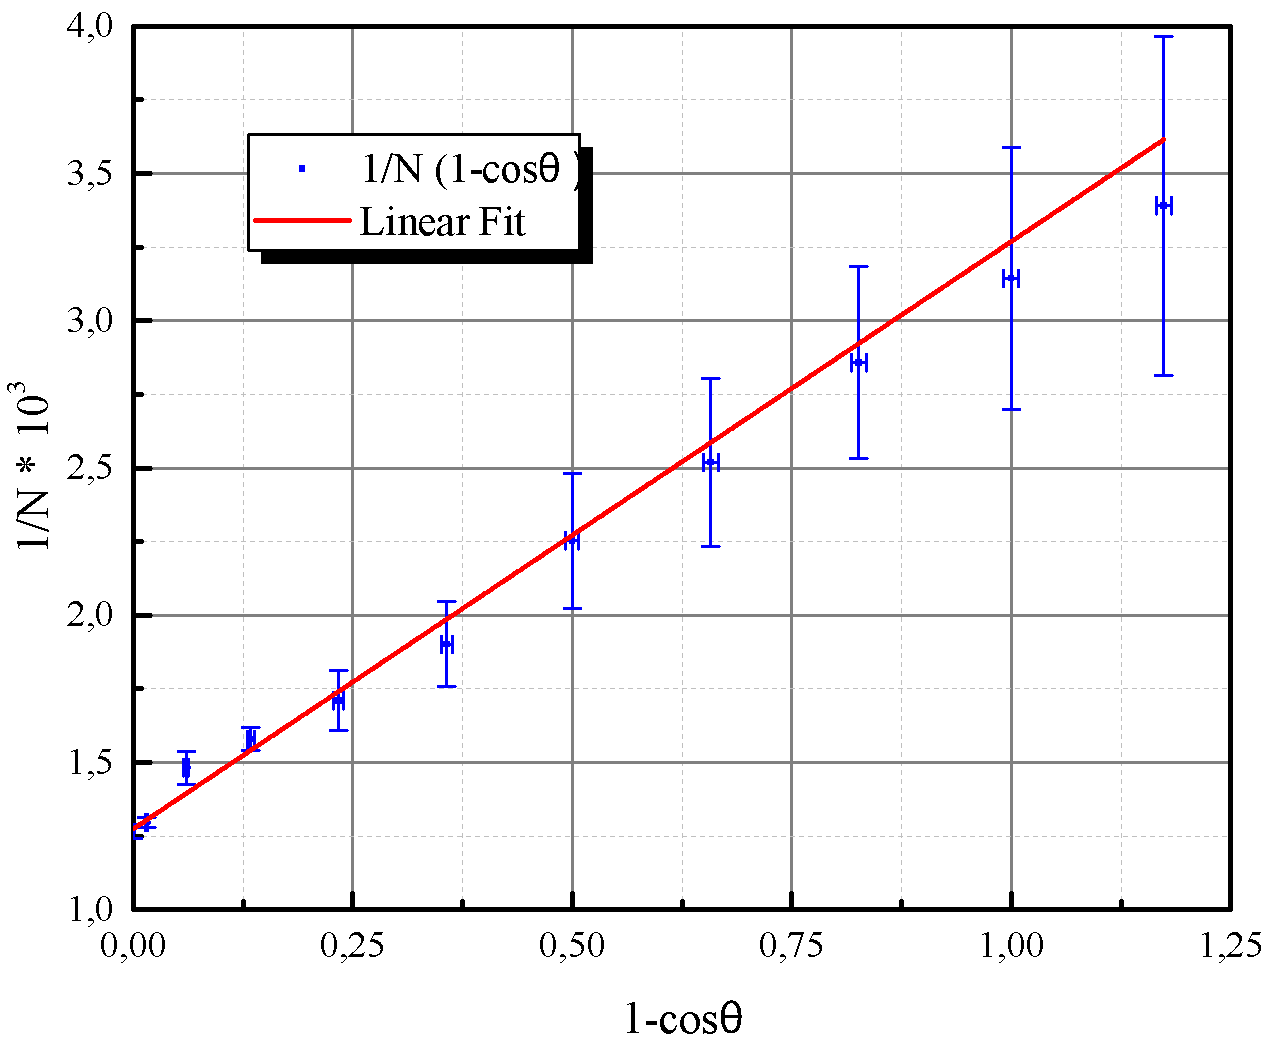
\includegraphics[width=1\textwidth]{Graphics/graph1.png}}
\caption[]{\label{} График №1}
\end{figure}
Коэффициент наклона графика №1 $k_1 = 4,950 \pm 0,024 (\varepsilon = 0,49\%)$

\item Завершив первую серию измерений, охладим калориметр до комнатной температуры, достигнув нулевого напряжения на термопаре.

\item Повторим измерения для другого расхода. $q_2 \approx 0,1054 \pm 0,0003\frac{\text{г}}{\text{c}} (\varepsilon = 0,33\%)$
\clearpage
\begin{table}[h!] 
	\caption{Измерение $\Delta T (N) \; {при} \; q_2 = 0,1054 \pm 0,0003 \frac{\text{г}}{\text{c}}$}
	\begin{center}
		\begin{tabular}{|*{6}{c|}}
			\hline
			\textnumero & $U, \text{B} $ & $\varepsilon,  \text{мВ}$ & $I, \text{мА}$ & $\Delta T, ^\circ\text{C}$ & $N,  \text{Вт} $\\ \hline
			1	&1,9	&0,036&	53,13	&0,88	&0,101 \\ \hline
			2	&2,98	&0,082&	83,15	&2,01	&0,248\\ \hline
			3	&4,2	&0,163	&117,64	&4,00	&0,494\\ \hline
			4	&5,15	&0,241&	143,97&	5,92&	0,741\\ \hline
			5	&5,95	&0,325	&166,18	&7,99&	0,989\\ \hline
			6	&6,66	&0,405	&186,12&9,95	&1,240\\ \hline
		\end{tabular}
	\end{center}
\end{table}


\begin{figure}[h!]
\centering{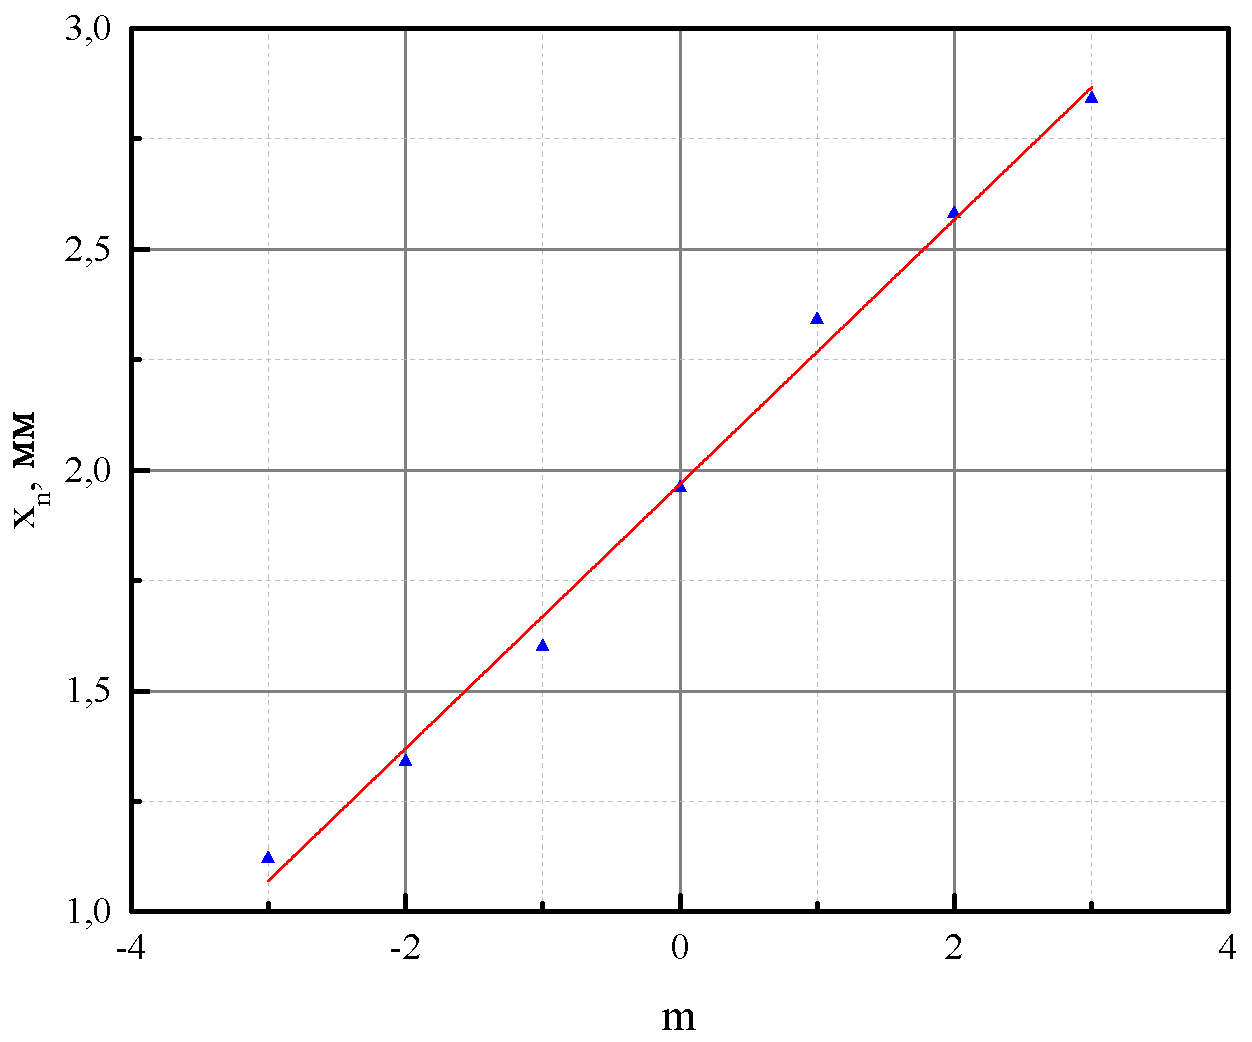
\includegraphics[width=1\textwidth]{Graphics/graph2.png}}
\caption[]{\label{fig:3} График №2}
\end{figure}

Коэффициент наклона графика №1 $k_2 = 8,044 \pm 0,022 (\varepsilon = 0,27\%)$ \newline



\item Найдем $c_{p}$ и $\alpha$, используя формулу (7).
\begin{equation*}
	c_{p} = \frac{\frac{1}{k_1}-\frac{1}{k_2}}{q_1-q_2} = 0,942 \pm 0,013 \frac{\text{Дж}}{г\cdot K} (\varepsilon = 1,38\%)
\end{equation*}
\begin{equation*}
	\alpha = \frac{\frac{q_1}{k_2} - \frac{q_2}{k_1}}{q_1-q_2} = 0,0249 \pm 0,0037 \frac{\text{Вт}}{K}(\varepsilon = 14,79\%)
\end{equation*}

\item По формуле (6) определим долю тепловых потерь $\frac{N_{\text{пот}}}{N}$в опыте

\begin{table}[h!] 
	\caption{Доля тепловых потерь $\frac{N_{\text{пот}}}{N}$в 1 серии}
	\begin{center}
		\begin{tabular}{|*{6}{c|}}
			\hline
			$N,  \text{Вт} $ & $N_{\text{пот}}, \text{Вт}$ & $\Delta N_{\text{пот}}, \text{Вт}$ & $\frac{N_{\text{пот}}}{N}, \%$ & $\Delta \frac{N_{\text{пот}}}{N}$ & $\varepsilon_{\frac{N_{\text{пот}}}{N}}, \%$\\ \hline
			0,182	&0,0239&	0,0035	&13,1	&0,038	&29,3\\ \hline
			0,366	&0,0466	&0,0069	&12,7	&0,032	&25,0\\ \hline
			0,714	&0,0876&	0,0130	&12,3&	0,027&	22,1\\ \hline
			1,100	&0,1329	&0,0197	&12,1	&0,025&	20,7\\ \hline
			1,389	&0,1734&	0,0257	&12,5 &	0,025&	20,1\\ \hline
			1,737	&0,2144&	0,0317&	12,3 &	0,024&	19,5\\ \hline
		\end{tabular}
	\end{center}
\end{table}

\begin{table}[h!] 
	\caption{Доля тепловых потерь $\frac{N_{\text{пот}}}{N}$во 2 серии}
	\begin{center}
		\begin{tabular}{|*{6}{c|}}
			\hline
			$N,  \text{Вт} $ & $N_{\text{пот}}, \text{Вт}$ & $\Delta N_{\text{пот}}, \text{Вт}$ & $\frac{N_{\text{пот}}}{N}, \%$ & $\Delta \frac{N_{\text{пот}}}{N}$ & $\varepsilon_{\frac{N_{\text{пот}}}{N}}, \%$\\ \hline
			0,101&	0,0221&	0,0033&21,8 &	0,075&	34,4\\ \hline
			0,248&	0,0502&	0,0074&	20,3 &	0,055&	27,3\\ \hline
			0,494&	0,0999&	0,0148&	20,2 &	0,048&	23,6\\ \hline
			0,741&	0,1476&	0,0218&	19,9 &	0,044&	22,0\\ \hline
			0,989&	0,1991&	0,0295&20,1 &	0,042&	21,0\\ \hline
			1,240&	0,2481&	0,0367&	20,0 &	0,041&	20,4\\ \hline
					\end{tabular}
	\end{center}
\end{table}

\section{Итог}
Сравним полученное значение удельной теплоемкости воздуха с табличными значениями (сравниваем с сухим воздухом)

\begin{table}[h!] 
	\caption{Сравнение }
	\begin{center}
		\begin{tabular}{|*{6}{c|}}
			\hline
			& $c_{p}, \frac{\text{Дж}}{г\cdot K}$ & $\Delta c_{p}, \frac{\text{Дж}}{г\cdot K}$ & $\varepsilon_{c_{p}}, \%$ \\ \hline
			эксперементальное & 0,942&	0,013	&1,38\\ \hline
			теоретическое&1,002	&0,059&5,97\\ \hline
			табличное&0,992	&0,049	&5,03\\ \hline
		\end{tabular}
	\end{center}
\end{table}
\section{Выводы}
Используя оборудование экспериментальной установки и законы термодинамики, мы получили значение удельной теплоемкости воздуха при постоянном давлении. Оно равно $c_{p} = 0,942 \pm 0,013 \frac{\text{Дж}}{г\cdot K} (\varepsilon = 1,38\%)$. С табличным и теоретическим значениями оно расходится не более чем на 6\%. Могу предположить, что погрешность обусловлена погрешностью оборудования, а также теоретическими апроксимациями: мы считали, что воздух - идеальный двухатомный газ. Для установления идеального равновесия 
требуется много времени, из-за чего результаты напряжения на термопаре не идеально точные. Также из-за влажности воздуха теоретическая удельная теплоемкость должна быть больше, что говорит о большем потенциальном расхождении.
Были получены примерные тепловые потери для каждой серии измерений. В первой потери составляют 12,5 \% в среднем (максимальная погрешность 29,3 \%), во второй 20,4\% (34,4\%). Как мы видим, потери увеличиваются с увеличением расхода воздуха. Высокая погрешность обусловлена неравновесностью системы, а также апроксимацией формулы для потерь.
\end{enumerate}
\end{document}